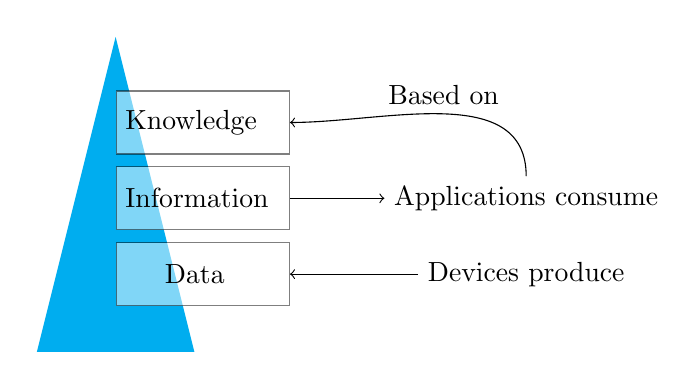
\begin{tikzpicture}
	\fill[cyan] (0,0) node (a) {} 
	-- (-1,-4) node (b) {} 
	-- node[pos=0.5,inner sep=0pt] (bc) {} (1, -4) node {} 
	-- cycle;
	\draw[cyan] (a) -- node[pos=0.25] (a1) {} node[pos=0.5] (a2) {} node[pos=0.75] (a3) {} (bc);
	\draw (a3) node[rectangle, draw, right, fill=white, opacity=0.5, minimum width=2.2cm, minimum height=0.8cm] (data) {};
	\draw (a3) node[right, xshift=0.5cm] {Data};
	\draw (a2) node[rectangle, draw, right, fill=white, opacity=0.5, minimum width=2.2cm, minimum height=0.8cm] (info) {};
	\draw (a2) node[right] {Information};
	\draw (a1) node[rectangle, draw, right, fill=white, opacity=0.5, minimum width=2.2cm, minimum height=0.8cm] (knowledge){};
	\draw (a1) node[right] {Knowledge};
	
	\draw ([xshift=3cm]data.east) node (devices) {Devices produce};
	\draw[->] (devices) -- (data);
	\draw ([xshift=3cm]info.east) node (app) {Applications consume};
	\draw[<-] (app) -- (info);
	\draw[->] (app.north) to[out=90, in=0] node[above] {Based on} (knowledge.east);
\end{tikzpicture}